\begin{figure}
  \centering
    \includegraphics[width=0.75\textwidth]{Figures/p_vs_K_fm.pdf}
  \caption{Reproduction of Figure 12b of Flache and Macy (2011). The average
    polarization decreases with $K$. However, as shown in subsequent figures,
    this does not mean trials with high polarization never obtain. Average
    taken over 100 trials.
  }
  \label{fig:p_vs_K_fm}
\end{figure}


\begin{figure}[h!]
  \centering
    \begin{subfigure}[t]{\textwidth}
      \centering
      \includegraphics[width=.55\textwidth]{Figures/connected-caveman-over-K.pdf}
      \caption{Non-random connected caveman network.}
      \label{fig:connected-caveman-trials}
    \end{subfigure}
    \begin{subfigure}[t]{\textwidth}
      \centering
      \includegraphics[width=.55\textwidth]{Figures/random-shortrange-over-K.pdf}
      \caption{Random connected caveman network with short-range random ties added at iteration 2000.}
      \label{fig:random-shortrange-trials}
    \end{subfigure}
    \begin{subfigure}[t]{\textwidth}
      \centering
      \includegraphics[width=.55\textwidth]{Figures/random-anyrange-over-K.pdf}
      \caption{Randomized connected caveman network with long-range random ties added at iteration 2000.}
      \label{fig:random-anyrange-trials}
    \end{subfigure}
  \caption{Results of indivdual model runs for different network conditions. 
    The averages of these were shown in Figure~\ref{fig:p_vs_K_fm}.
    Even in the non-random connected caveman structure, there is 
    variation in the final polarization for different values of $K$. Highly
    polarized final states may obtain. 100 trials are shown for each 
    network condition and comprise the
    average. The circled square in~\ref{fig:connected-caveman-trials}
    highlights the experimental configuration
    reused to make Figure~\ref{fig:highpol-histogram}.
  }
  \label{fig:single-experiments-over-k}
\end{figure}


\begin{figure}[h!]
  \centering
    \includegraphics[width=.75\textwidth]{Figures/final-initial-pol-regplot.pdf}
  \caption{Regression of final polarization against initial polarization 
    for $K=2$ in the non-random connected caveman network configuration.
    Final polarizations are same as in the $K=2$ column of 
    Figure~\ref{fig:connected-caveman-trials}. 100 trials are shown. The
    top histogram shows the distribution of initial polarization across
    trials. The right histogram shows the distribution of final polarization
    across trials.}
  \label{fig:final-initial-pol-regplot}
\end{figure}

\begin{figure}[h!]
  \centering
    \includegraphics[width=.75\textwidth]{Figures/caveman-highpol-histogram-10k-its.pdf}
  \caption{Distribution of final polarizations at iteration 10000
  starting from initial conditions of the connected caveman trial with 
  maximal final polarization for $K=2$ shown in 
  Figure~\ref{fig:connected-caveman-trials}.
  The distribution is skewed towards final polarizations considerably larger
  than the mean polarization of 0.41 for the connected caveman experiment
  with $K=2$ found by Flache and Macy and shown in Figure~\ref{fig:p_vs_K_fm}. 
  }
  \label{fig:highpol-histogram}
\end{figure}

% \begin{figure}[t!]
%   \centering
%   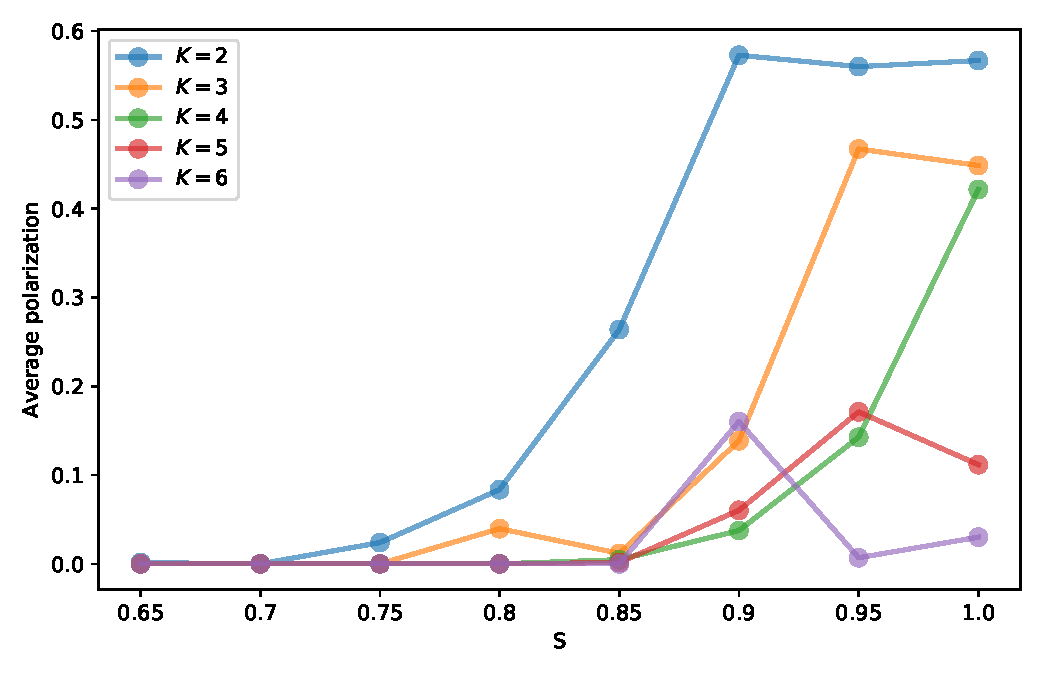
\includegraphics[width=0.75\textwidth]{Figures/P_vs_S_for_K.pdf}
%   \caption{
%     Average final polarization becomes non-zero then increases as
%     the width of the uniform distribution of initial opinions increases.
%     The width must be larger and larger as the cultural complexity $K$ 
%     increases for the system to achieve non-zero final polarization. This
%     condition is identical to the bottom row of each heatmap in 
%     Figure \ref{fig:heatmaps}. Each
%     data point is the average of fifty trials. Each trial ran over 
%     10k timesteps. 
%   }
%   \label{fig:p_vs_s_for_k}
% \end{figure}


\begin{figure}[t!]
  \centering
    \includegraphics[width=0.75\textwidth]{Figures/s_k_zoom_2-6_mean.pdf}
  \caption{Average polarization for different cultural complexities over 
    maximum initial opinion magnitude, $S$. 
    Averages are roughly zero for $S<0.75$ for all cultural complexities.
    Each data point is the average over 100 trials of the condition
    where long-range ties were added at iteration 2000. Each trial was run to 
    10k total iterations. 
  }
  \label{fig:S_average}
\end{figure}

\begin{figure}[h!]
  \centering
    \includegraphics[width=0.75\textwidth]{Figures/s_k_zoom_2-6_median.pdf}
  \caption{Median polarization for different cultural complexities over
    maximum initial opinion magnitude, $S$.
    Median polarization for $K=5$ and $K=6$ are both flat at zero; $K=5$ 
    data is obscured by $K=6$.  Median taken over 100 trials.
    Same data as in Figure~\ref{fig:S_average}, so the condition was
    long-range ties added at iteration 2000, with each trial run to 10k
    total iterations.
  }
  \label{fig:S_median}
\end{figure}


\begin{figure}[h!]
  \centering
  \begin{subfigure}[t]{\textwidth}
    \centering
    \includegraphics[width=0.5\textwidth]{Figures/single_S_K=2.pdf}
  \end{subfigure} \\
  \begin{subfigure}[t]{0.49\textwidth}
      \centering
      \includegraphics[width=\textwidth]{Figures/single_S_K=3.pdf}
      % \caption{}
  \end{subfigure}
  ~
  \begin{subfigure}[t]{0.49\textwidth}
      \centering
      \includegraphics[width=\textwidth]{Figures/single_S_K=4.pdf}
      % \caption{}
  \end{subfigure} \\
  \begin{subfigure}[t]{0.49\textwidth}
      \centering
      \includegraphics[width=\textwidth]{Figures/single_S_K=5.pdf}
      % \caption{}
  \end{subfigure}
  ~
  \begin{subfigure}[t]{0.49\textwidth}
      \centering
      \includegraphics[width=\textwidth]{Figures/single_S_K=6.pdf}
      % \caption{}
  \end{subfigure}
  \caption{Final polarization of individual trial runs and averages from
    Figure~\ref{fig:S_average}. Each trial was run in the condition 
    where random long-range ties were added at iteration 2000 and each trial
    was run to 10k iterations.
  }
  \label{fig:single_S_K}
\end{figure}


\begin{figure}
  \centering
    \includegraphics[width=.75\textwidth]{Figures/min_parallel_K=2.pdf}
  \caption{}
  \label{fig:}
\end{figure}

\begin{figure}
  \centering
    \includegraphics[width=.75\textwidth]{Figures/max_parallel_K=2.pdf}
  \caption{}
  \label{fig:}
\end{figure}



\begin{figure}[t!]
  \centering
      \begin{subfigure}[t]{0.49\textwidth}
          \centering
          \includegraphics[width=\textwidth]{Figures/noisecomm_K=2.pdf}
          % \caption{}
      \end{subfigure}
      ~
      \begin{subfigure}[t]{0.49\textwidth}
          \centering
          \includegraphics[width=\textwidth]{Figures/noisecomm_K=3.pdf}
          % \caption{}
      \end{subfigure} \\
      \begin{subfigure}[t]{0.49\textwidth}
          \centering
          \includegraphics[width=\textwidth]{Figures/noisecomm_K=4.pdf}
          % \caption{}
      \end{subfigure}
      ~
      \begin{subfigure}[t]{0.49\textwidth}
          \centering
          \includegraphics[width=\textwidth]{Figures/noisecomm_K=5.pdf}
          % 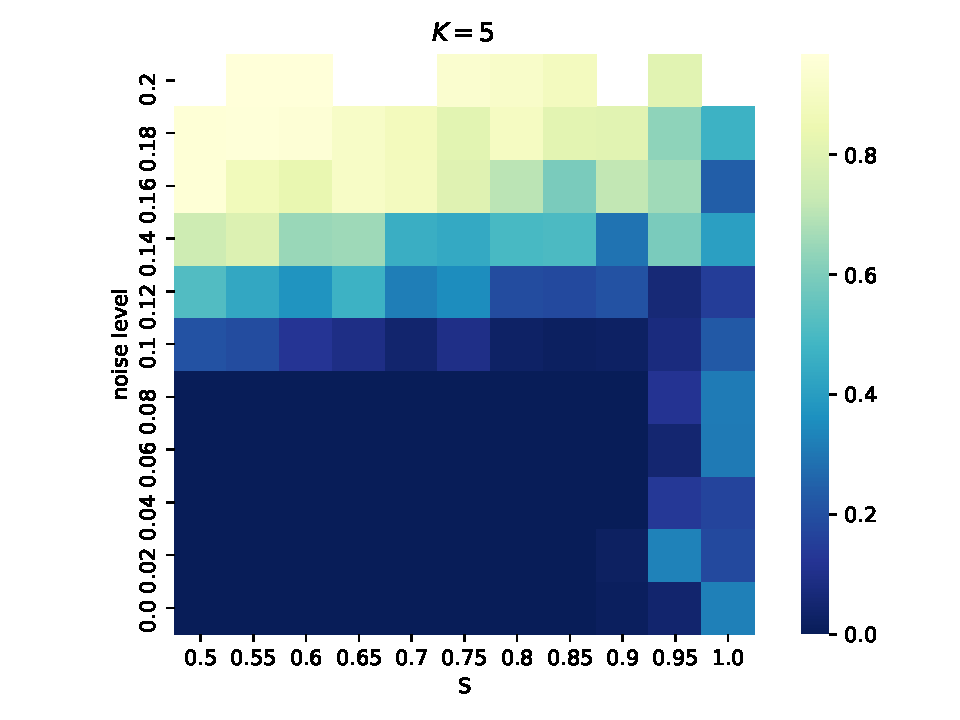
\includegraphics[width=\textwidth]{Figures/p_v_noise_k=5.pdf}
          % \caption{}
      \end{subfigure} \\
  \caption{Final average polarization varies with both the width of the
    uniform distribution of initial opinion magnitudes and the noise level in
    the opinion updates. The value in each square of the heatmap is the average of
    fifty trials. Each trial was run in the condition where random long-range
    ties were added at iteration 2000. Each trial ran to 10k timesteps. 
  }
  \label{fig:heatmaps}
\end{figure}


\begin{figure}[t!]
  \centering
      \begin{subfigure}[t]{0.49\textwidth}
          \centering
          \includegraphics[width=\textwidth]{Figures/noisecomm_S=0p5_K=2.pdf}
          % \caption{}
      \end{subfigure}
      ~
      \begin{subfigure}[t]{0.49\textwidth}
          \centering
          \includegraphics[width=\textwidth]{Figures/noisecomm_level=0p10_K=2.pdf}
          % \caption{}
      \end{subfigure} \\
      \begin{subfigure}[t]{0.49\textwidth}
          \centering
          \includegraphics[width=\textwidth]{Figures/noisecomm_S=0p5_K=4.pdf}
          % \caption{}
      \end{subfigure}
      ~
      \begin{subfigure}[t]{0.49\textwidth}
          \centering
          \includegraphics[width=\textwidth]{Figures/noisecomm_level=0p10_K=4.pdf}
          % \caption{}
      \end{subfigure} \\
      \begin{subfigure}[t]{0.49\textwidth}
          \centering
          \includegraphics[width=\textwidth]{Figures/noisecomm_S=0p5_K=6.pdf}
          % \caption{}
      \end{subfigure}
      ~
      \begin{subfigure}[t]{0.49\textwidth}
          \centering
          \includegraphics[width=\textwidth]{Figures/noisecomm_level=0p10_K=6.pdf}
          % \caption{}
      \end{subfigure}
  \caption{Final polarization of individual trial runs and averages from
    Figure~\ref{fig:heatmaps}. Each trial was run in the condition where
    random long-range ties were added at iteration 2000 and each trial was
    run to 10k iterations. In the left column, the maximum inintial opinion
    magnitude, $S$, is constant at 0.5 and noise level vaies along the x-axis. 
    As the noise level is increased, the
    system is increasingly biased towards larger final polarization outcomes.
    In the right column, the noise level is held constant at 0.1 and $S$ 
    varies along the x-axis. For cultural complexity of $K=6$, most trials do
    not attain large values of final polarization.
  }
  \label{fig:single-runs-commnoise}
\end{figure}
